\section{RQ2}
\label{sec:RQ2}
To understand where the learning signal settles in representation space, we investigate three aspects.
(1) \textbf{Accumulated Representation Adaptation}, which examines the magnitude, dominant directions, and stability of representation changes during training;
(2) \textbf{Representation-Space Gradient Dynamics}, which characterizes how the strength and directional distribution of hidden gradients change during training;
and (3) \textbf{Gradient Coverage by Early Adaptation Directions}, which measures how much gradient energy is captured by the subspace of early representation changes.
We use the paired FULL trajectories at both scales. Complete observations and metric definitions appear in Appendices~\ref{app:displacement} and~\ref{app:supplementary}.

\subsection{Accumulated Representation Adaptation}
\label{sec:rq2_adaptation}
We first examine how representation changes accumulate and whether their dominant directions persist. At each checkpoint, we evaluate the same fixed probe prefixes and extract the final hidden states. For a prefix $c$, define the unit-normalized state $\hat h_t(c)=h_t(c)/\|h_t(c)\|_2$ and its change from initialization,
\begin{equation}
 d_t(c)=\hat h_t(c)-\hat h_0(c),\qquad
 C_t=\frac{1}{N}\sum_c d_t(c)d_t(c)^\top.
 \label{eq:rq2_representation_change}
\end{equation}
Here $N$ is the number of probe positions. The RMS magnitude of representation change is $\sqrt{\operatorname{tr}(C_t)}$. For descending eigenvalues $\lambda_j(C_t)$, the energy captured by the leading $r$ directions of representation change is $D_t(r)=\sum_{j=1}^{r}\lambda_j(C_t)/\operatorname{tr}(C_t)$.

Cumulative representation change grows at both scales while retaining substantial spectral concentration (Figure~\ref{fig:rq2_adaptation}). Its final leading 128 directions cover 90.36\% of representation change energy in 1.7B and 84.14\% in 4B (Table~\ref{tab:rq2_summary}). The full spectrum also reveals a scale-dependent difference. The first direction accounts for over half of the energy in 1.7B, whereas 4B distributes more energy across subsequent directions. Concentration therefore extends across a range of ranks, with a stronger leading mode in the smaller model.

To examine persistence, we fix $U_{10}$ to the leading 128 eigenvectors of $C_{10}$ and measure $\operatorname{tr}(U_{10}^\top C_tU_{10})/\operatorname{tr}(C_t)$. This early basis continues to cover most cumulative representation change through the endpoint (Figure~\ref{fig:rq2_adaptation}c). Independent original FULL runs also show high overlap between subspaces of representation change at late checkpoints, measured by $\|U_a^\top U_b\|_F^2/128$ for two checkpoint bases (Appendix~\ref{app:displacement}, Table~\ref{tab:subspace}). Together, these measurements support persistent structure in accumulated adaptation. The fixed-basis coverage includes the first ten updates because representation change is always measured from initialization.

\begin{figure*}[t]
\centering
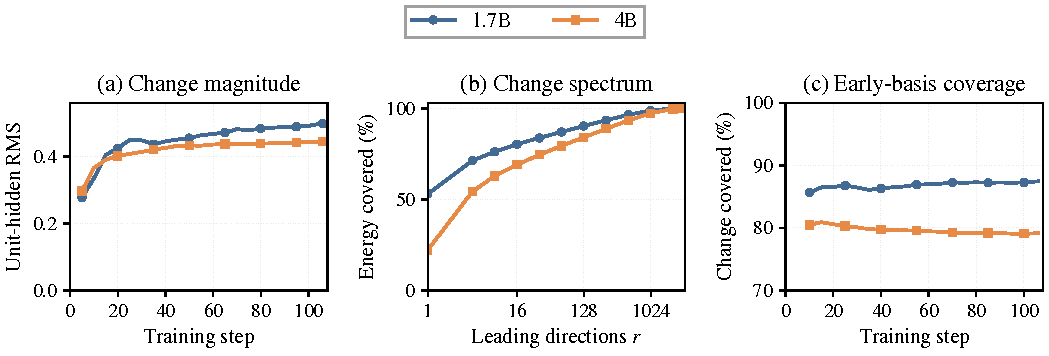
\includegraphics[width=\textwidth]{figures/rq2_adaptation.pdf}
\caption{Accumulated representation changes in paired FULL. (a) RMS change in unit-normalized hidden states from initialization, evaluated on fixed probe prefixes. (b) Cumulative representation change energy covered by the final checkpoint's own leading directions at step 106. The rank axis is logarithmic. (c) Coverage of cumulative representation change by the fixed step-10 rank-128 basis $U_{10}$. Markers identify the models. Lines connect recorded observations.}
\label{fig:rq2_adaptation}
\end{figure*}

\subsection{Representation-Space Gradient Dynamics}
\label{sec:rq2_gradients}
We next examine the supervision currently reaching the representation. With logits $z_t=W_th_t$, the individual-position hidden gradient is $g_{h,t}(c)=W_t^\top\nabla_{z_t}\ell_t(c)$.
Let $G_t$ contain these gradients as rows for the current sampled training responses, with $N_t$ positions and singular values $\sigma_{j,t}$. We summarize gradient strength by $\|G_t\|_F/\sqrt{N_t}$. To describe its distribution across directions, set $w_{j,t}=\sigma_{j,t}^2/\sum_k\sigma_{k,t}^2$ and compute
\begin{equation}
 H_t(r)=\sum_{j=1}^{r}w_{j,t},\qquad
 R_t=\exp\!\left(-\sum_jw_{j,t}\log w_{j,t}\right).
 \label{eq:rq2_gradient_spectrum}
\end{equation}
Here $H_t(r)$ is cumulative gradient-energy coverage and $R_t$ is energy effective rank.

The current signal weakens as its normalized energy distribution becomes more spread out (Figure~\ref{fig:rq2_gradients}). Between the first and final observations, gradient RMS decreases at both scales, while effective rank increases from 110.16 to 303.36 in 1.7B and from 87.41 to 371.55 in 4B (Table~\ref{tab:rq2_summary}). The intermediate measurements show fluctuations around this broad change. The final gradient spectra still have prominent leading directions, although these directions cover less energy than equally sized subspaces of representation change. 
\begin{figure*}[t]
\centering
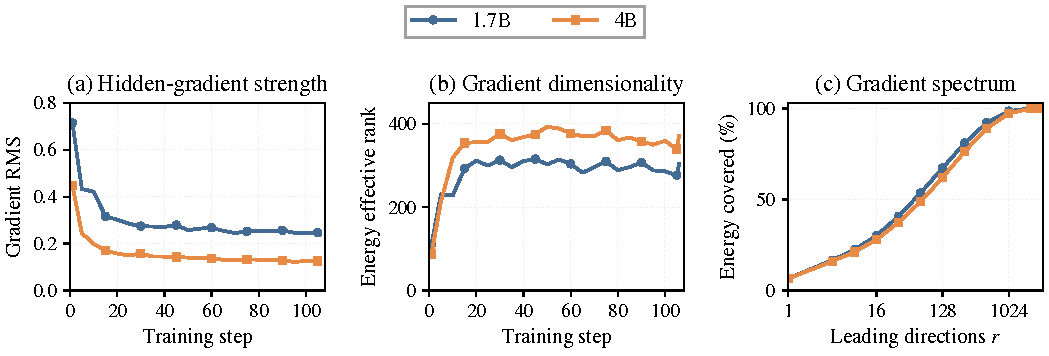
\includegraphics[width=\textwidth]{figures/rq2_gradient_dynamics.pdf}
\caption{Current hidden-gradient structure in paired FULL. (a) Per-position gradient RMS and (b) energy effective rank over training. (c) Cumulative gradient energy captured by the current gradient matrix's own leading directions at step 106. All panels use the full hidden space and sampled training responses. Lines connect measured observations. The spectrum uses a logarithmic rank axis.}
\label{fig:rq2_gradients}
\end{figure*}

\subsection{Gradient Coverage by Early Adaptation Directions}
\label{sec:rq2_coverage}
Although we have examined accumulated representation changes
and hidden-gradient dynamics separately, it remains unclear
whether the remaining gradient energy is concentrated along
the directions established during early representation adaptation.
To answer this question, we project the hidden gradients onto
the fixed early adaptation subspace $U_{10}$ and measure the
fraction of gradient energy it captures,
\begin{equation}
 A_t=\frac{\|G_tU_{10}\|_F^2}{\|G_t\|_F^2}.
 \label{eq:rq2_gradient_coverage}
\end{equation}
At the endpoint, $U_{10}$ covers 87.46\% and 79.16\% of accumulated representation change energy in 1.7B and 4B, respectively, and 16.71\% and 15.18\% of current gradient energy (Figure~\ref{fig:rq2_coverage}). Most current gradient energy therefore lies outside these early adaptation directions.

An equal-rank comparison clarifies the role of direction choice. The current gradients' own leading 128 directions capture 67.31\% and 62.12\% of their energy at the two scales, substantially exceeding coverage by $U_{10}$ (Table~\ref{tab:rq2_summary}). Current supervision retains concentrated directions, while the early adaptation basis provides limited coverage of those gradients. The comparisons use fixed probe prefixes for representation change and current sampled responses for gradients, with $U_{10}$ held identical across the two measurements. They establish how current sensitivity is distributed relative to historical adaptation. The effect of an executed update on unseen responses is examined in RQ3.

\begin{figure*}[t]
\centering
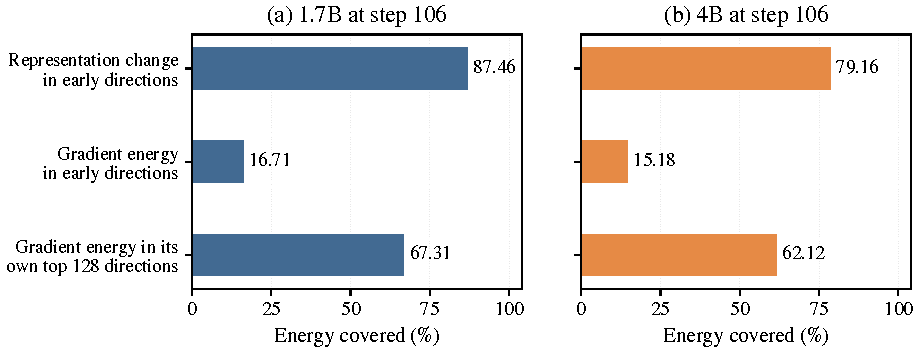
\includegraphics[width=0.85\textwidth]{figures/rq2_gradient_coverage.pdf}
\caption{Representation changes and hidden-gradient directions at the end step. We identify the top 128 directions of accumulated representation change at step 10 and keep them fixed. These early directions capture most of the accumulated representation change, but only a small fraction of the hidden-gradient energy at step 106. For comparison, the third bar shows the gradient energy captured by the gradient's own top 128 directions. Representation changes are measured on fixed probe prefixes, while gradients are measured on sampled training responses.}
\label{fig:rq2_coverage}
\end{figure*}

\begin{table}[t]
\centering
\caption{Core paired FULL representation results. Arrows give the first and last stated observations. Coverage entries are percentages. Full trajectories and spectra appear in Appendices~\ref{app:displacement} and~\ref{app:supplementary}.}
\label{tab:rq2_summary}
\footnotesize
\setlength{\tabcolsep}{2pt}
\begin{tabular}{lrr}
\toprule
Measurement & 1.7B & 4B \\
\midrule
\multicolumn{3}{l}{\textit{Representation change, step 10 $\to$ 106}}\\
Unit-hidden RMS & $.3350\to.4984$ & $.3657\to.4457$\\
Own-1 coverage & $38.81\to53.02$ & $22.90\to22.24$\\
Own-128 coverage & $85.66\to90.36$ & $80.50\to84.14$\\
Fixed-$U_{10}$ coverage & $85.66\to87.46$ & $80.50\to79.16$\\
\midrule
\multicolumn{3}{l}{\textit{Hidden gradients, step 1 $\to$ 106}}\\
RMS & $.7149\to.2397$ & $.4469\to.1238$\\
Energy effective rank & $110.16\to303.36$ & $87.41\to371.55$\\
Own-128 coverage & $74.12\to67.31$ & $75.52\to62.12$\\
Fixed-$U_{10}$ coverage (106) & 16.71 & 15.18\\
\bottomrule
\end{tabular}
\end{table}
\FloatBarrier

\begin{tcolorbox}[
    enhanced,
    breakable,
    colback=findingbg,
    colframe=findingblue,
    boxrule=0.7pt,
    arc=1.5mm,
    left=7pt,
    right=7pt,
    top=6pt,
    bottom=6pt,
    before skip=8pt,
    after skip=8pt
]
\textbf{\textcolor{findingblue}{Key Finding}}
The teacher calls for changes across a much broader set of representation directions than those that dominate the student's accumulated changes. As training progresses, these correction signals become weaker and more spread out, while a small set of early directions continues to explain most of the accumulated representation change.
\end{tcolorbox}